\begin{frame}
\frametitle{Resultados - Grafos}

\begin{table}
	\caption{Cantidad de vértices, aristas y cliques de los grafos a comprimir.}
	\rowcolors{2}{white}{gray!10}
	\label{table:gafros1}
	\centering
	\footnotesize
	\begin{tabular}{l|r|r|r}
		\toprule
		Grafo & $|V|$ & $|E|$ & $|\mathcal{C}|$ \\
		\midrule
		marknewman-astro & 16.706 & 242.502 & 15.794 \\
		marknewman-condmat & 40.421 & 351.386 & 34.274 \\
		dblp-2010 & 326.186 & 1.615.400 & 196.434 \\
        dblp-2011 & 986.324 & 6.707.236 & 806.320 \\
		snap-dblp & 317.080 & 2.099.732 & 257.551 \\
        snap-amazon & 403.394 & 4.886.816 & 1.023.572 \\
        coPapersDBLP & 540.486 & 30.491.458 & 139.340 \\
        coPapersCiteseer & 434.102 & 32.073.440 & 86.303 \\
    	\bottomrule
	\end{tabular}
\end{table}

\end{frame}

\begin{frame}
\frametitle{Resultados - Grafos (2)}

\begin{table}
	\caption{Grado medio y máximo de los vértices, degeneracy, coeficiente de clusterización y transitividad de los grafos a comprimir.}
	\rowcolors{2}{white}{gray!10}
	\label{table:gafros2}
	\centering
	\footnotesize
	\begin{tabular}{l|r|r|r|r|r}
		\toprule
		Grafo & $\overline{d}$ & $d_{max}$ & $D(G)$ & $C(G)$ & $T(G)$ \\
		\midrule
		marknewman-astro & 14,51 & 360 & 56 & 0,66 & 0,42  \\
		marknewman-condmat & 8,69 & 278 & 29 & 0,64 & 0,24 \\
		dblp-2010 & 4,95 & 238 & 74 & 0,61 & 0,39  \\
        dblp-2011 & 6,80 & 979 & 118 & 0,63 & 0,20 \\
		snap-dblp & 6,62 & 2.752 & 113 & 0,63 & 0,30 \\
        snap-amazon & 12,11 & 343 & 10 & 0,41 & 0,16 \\
        coPapersDBLP & 56,41 & 3.299 & 336 & 0,80 & 0,65 \\
        coPapersCiteseer & 73,88 & 1.188 & 844 & 0,83 & 0,77 \\
    	\bottomrule
	\end{tabular}
\end{table}

\end{frame}


%% Distribución grado
\begin{frame}
\frametitle{Resultados - Distribución del grado de grafos}

\begin{figure}
    \centering
    	\begin{minipage}{1\textwidth}
    		\centering
    		\begin{minipage}{0.45\textwidth}
    			\centering
    			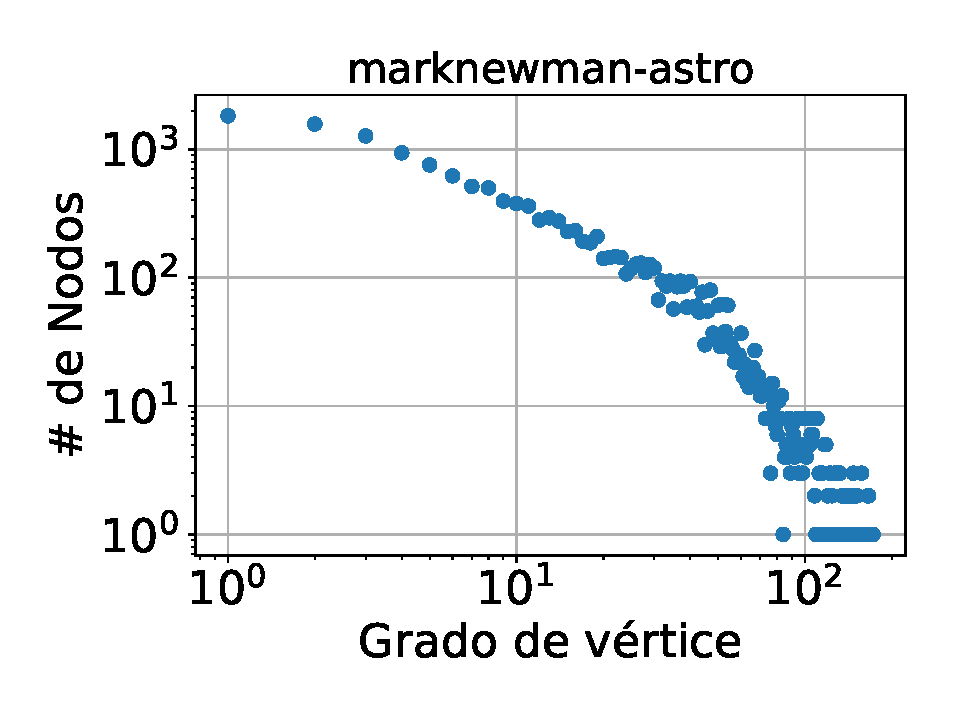
\includegraphics[width=1\linewidth]{../img/grades/marknewman-astro.pdf}
    		\end{minipage}
    		\begin{minipage}{0.45\textwidth}
    			\centering
    			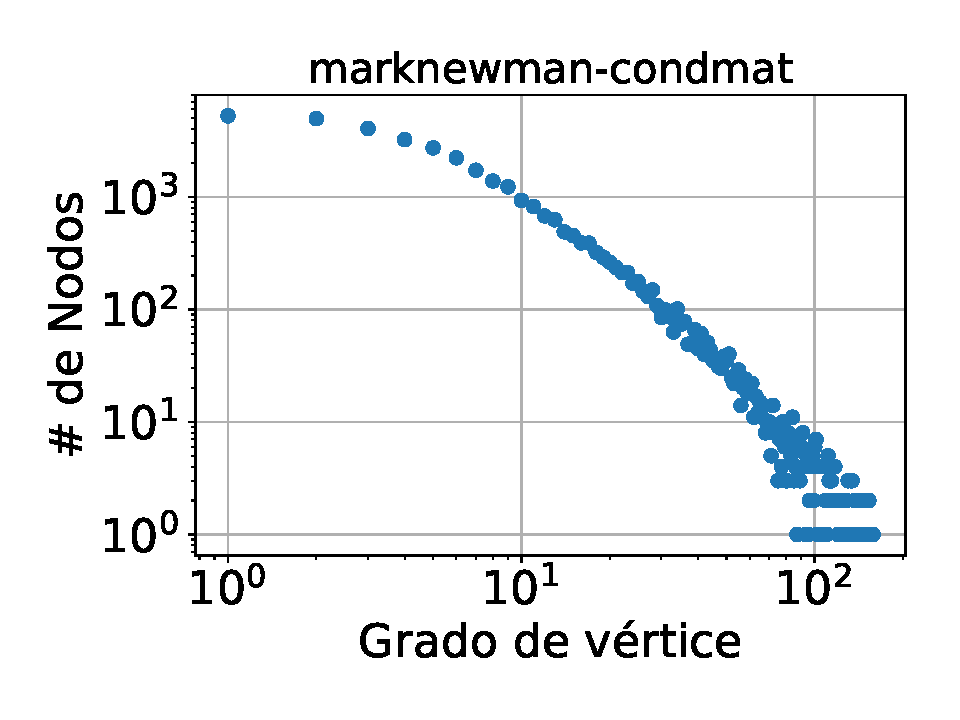
\includegraphics[width=1\linewidth]{../img/grades/marknewman-condmat.pdf}
    		\end{minipage}  		
    	\end{minipage}
    	
    	\begin{minipage}{1\textwidth}
    		\centering
    		\begin{minipage}{0.45\textwidth}
    			\centering
    			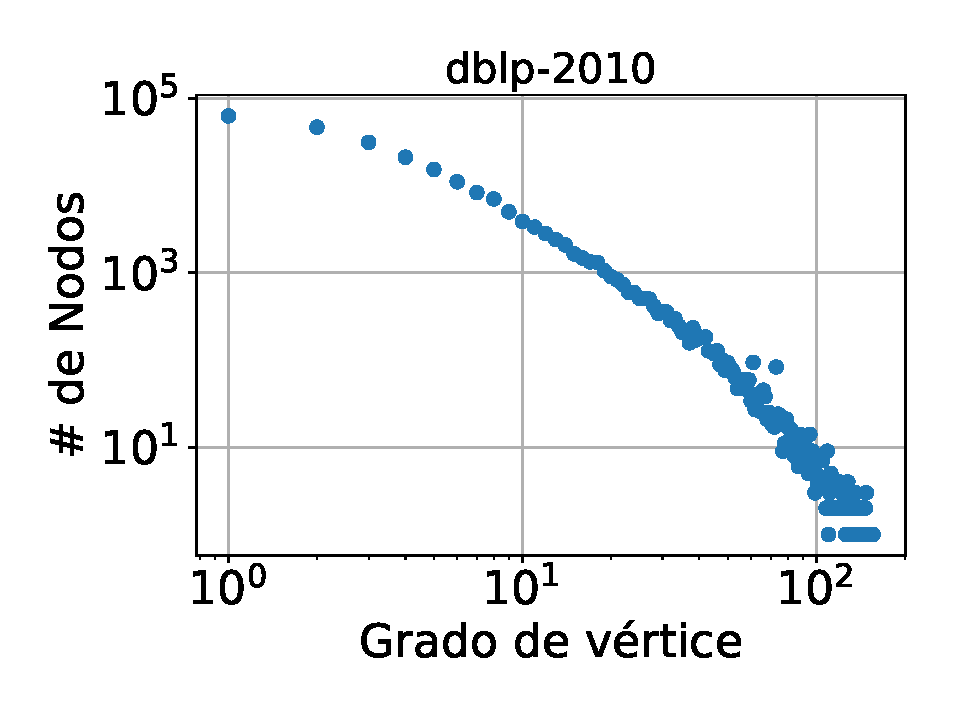
\includegraphics[width=1\linewidth]{../img/grades/dblp-2010.pdf}
    		\end{minipage}
    		\begin{minipage}{0.45\textwidth}
    			\centering
    			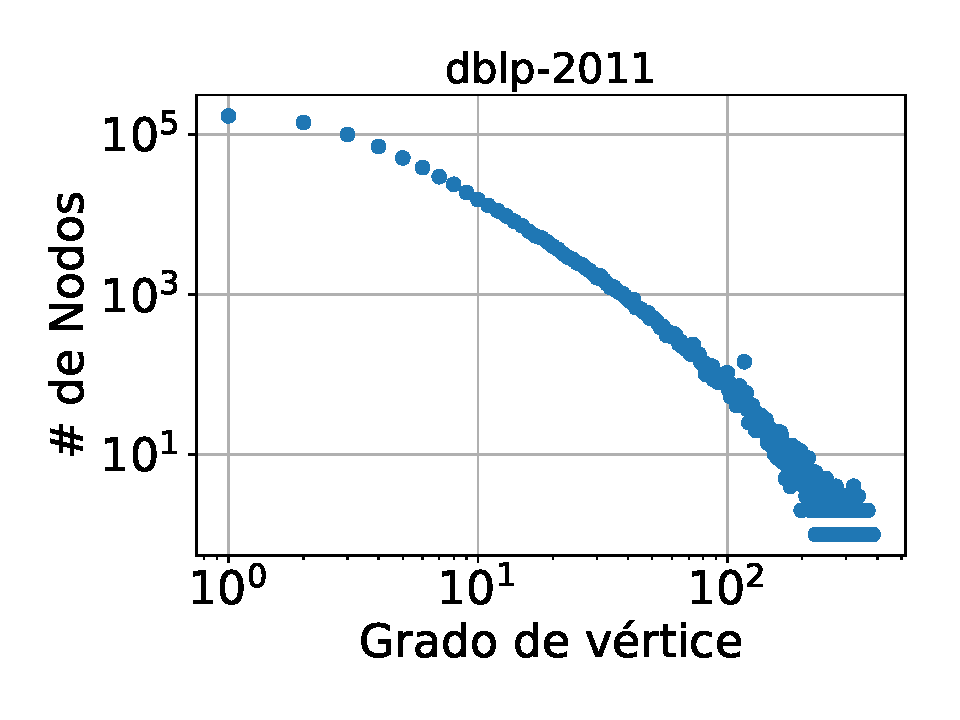
\includegraphics[width=1\linewidth]{../img/grades/dblp-2011.pdf}
    		\end{minipage}  
    	\end{minipage}	

    \caption{Distribución del grado de los vértices para cada grafo (1).}
\end{figure}


\end{frame}
\begin{frame}%[noframenumbering]
\frametitle{Resultados - Distribución del grado de grafos (2)}

\begin{figure}
    \centering
    	\begin{minipage}{1\textwidth}
    		\centering
    		\begin{minipage}{0.45\textwidth}
    			\centering
    			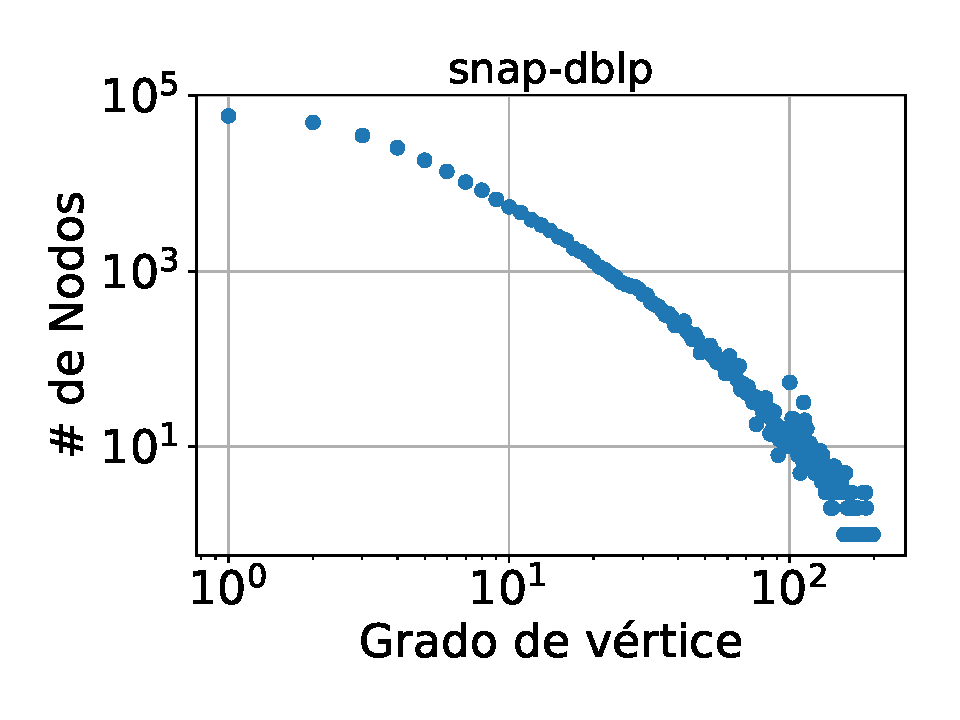
\includegraphics[width=1\linewidth]{../img/grades/snap-dblp.pdf}
    		\end{minipage}
    		\begin{minipage}{0.45\textwidth}
    			\centering
    			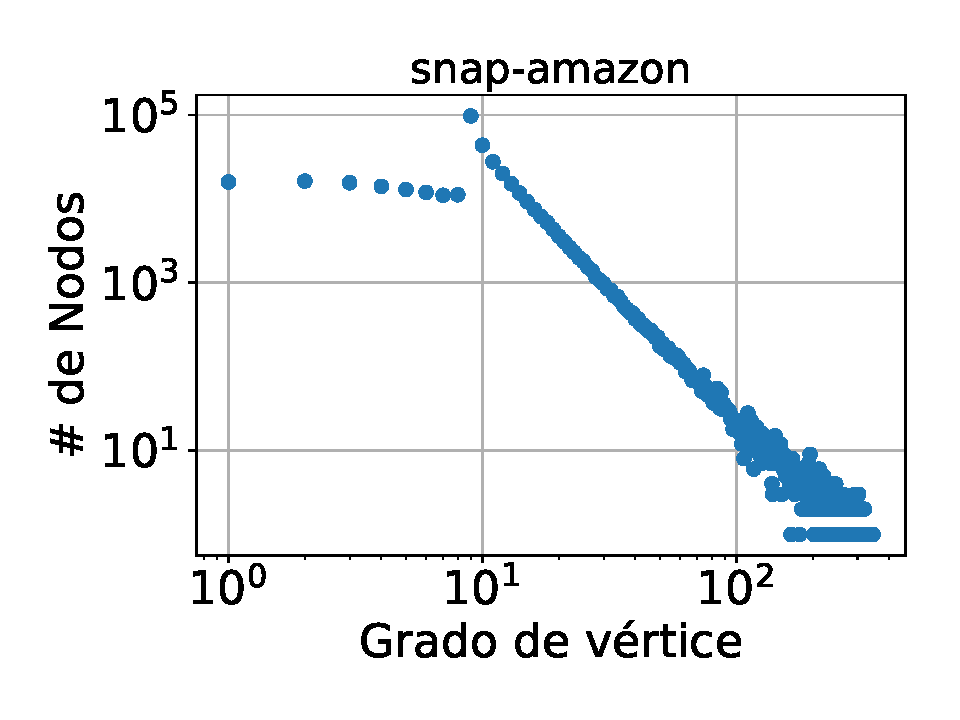
\includegraphics[width=1\linewidth]{../img/grades/snap-amazon.pdf}
    		\end{minipage}  		
    	\end{minipage}
    	
    	\begin{minipage}{1\textwidth}
    		\centering
    		\begin{minipage}{0.45\textwidth}
    			\centering
    			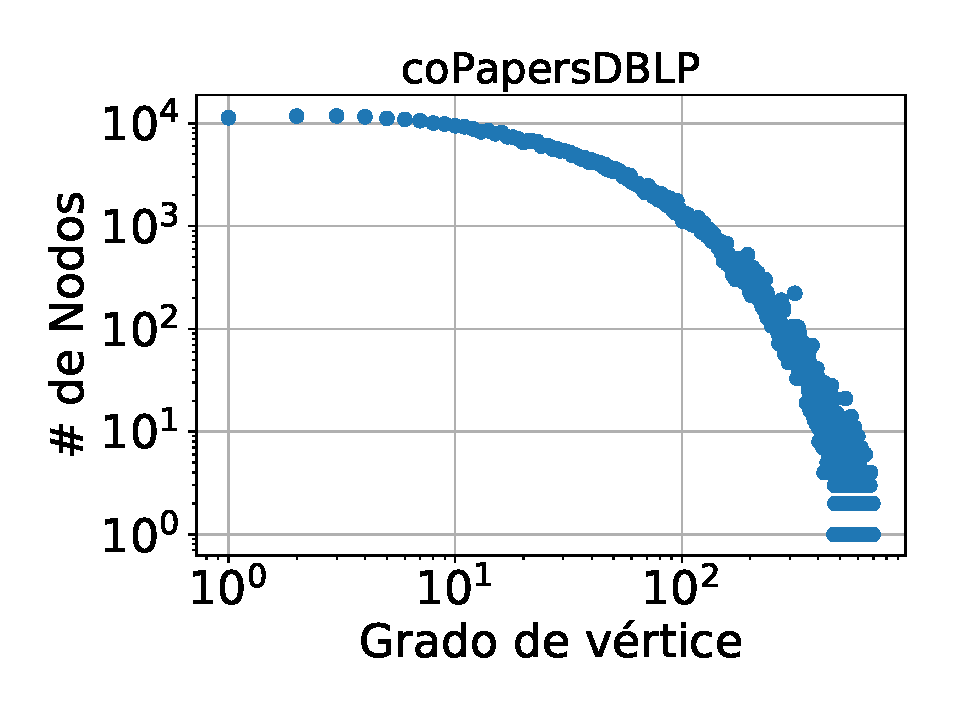
\includegraphics[width=1\linewidth]{../img/grades/coPapersDBLP.pdf}
    		\end{minipage}
    		\begin{minipage}{0.45\textwidth}
    			\centering
    			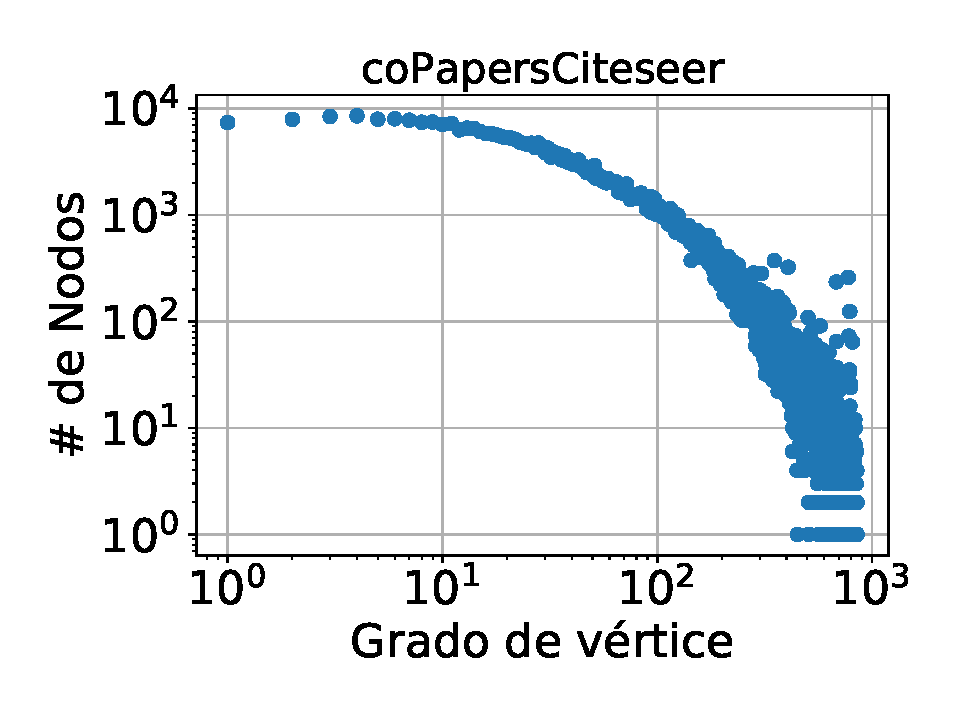
\includegraphics[width=1\linewidth]{../img/grades/coPapersCiteseer.pdf}
    		\end{minipage}  
    	\end{minipage}	

    \caption{Distribución del grado de los vértices para cada grafo (2).}
\end{figure}

\end{frame}





%% Estructura compacta
\begin{frame}
\frametitle{Resultados - Estructura compacta}

Se utiliza \texttt{SDSL}. Se seleccionan las siguientes estructuras:

\begin{itemize}
	\item Para las secuencias de símbolos $X$ e $Y$: estructuras basadas en wavelet matrix (\textit{wm}).
	\item Para la secuencia de bits $B$: estructuras basadas en bitmaps comprimidos de Raman, Raman y Rao (\textit{rrr}).
\end{itemize}

La secuencia de bytes $BB$ se comprime usando código Huffman.
\begin{itemize}
	\item Se actualizan índices en $Y$ para acceso por bits.
\end{itemize}

%Se evalúa nivel de compresión con respecto a acceso aleatorio y secuencial.

\end{frame}


%\begin{frame}
%\frametitle{Resultados - Estructura compacta(2)}
%
%\begin{figure}
%	\centering
%	
%    	\begin{minipage}{1\textwidth}
%    		\centering
%    		\begin{minipage}{0.8\textwidth}
%    			\centering
%    			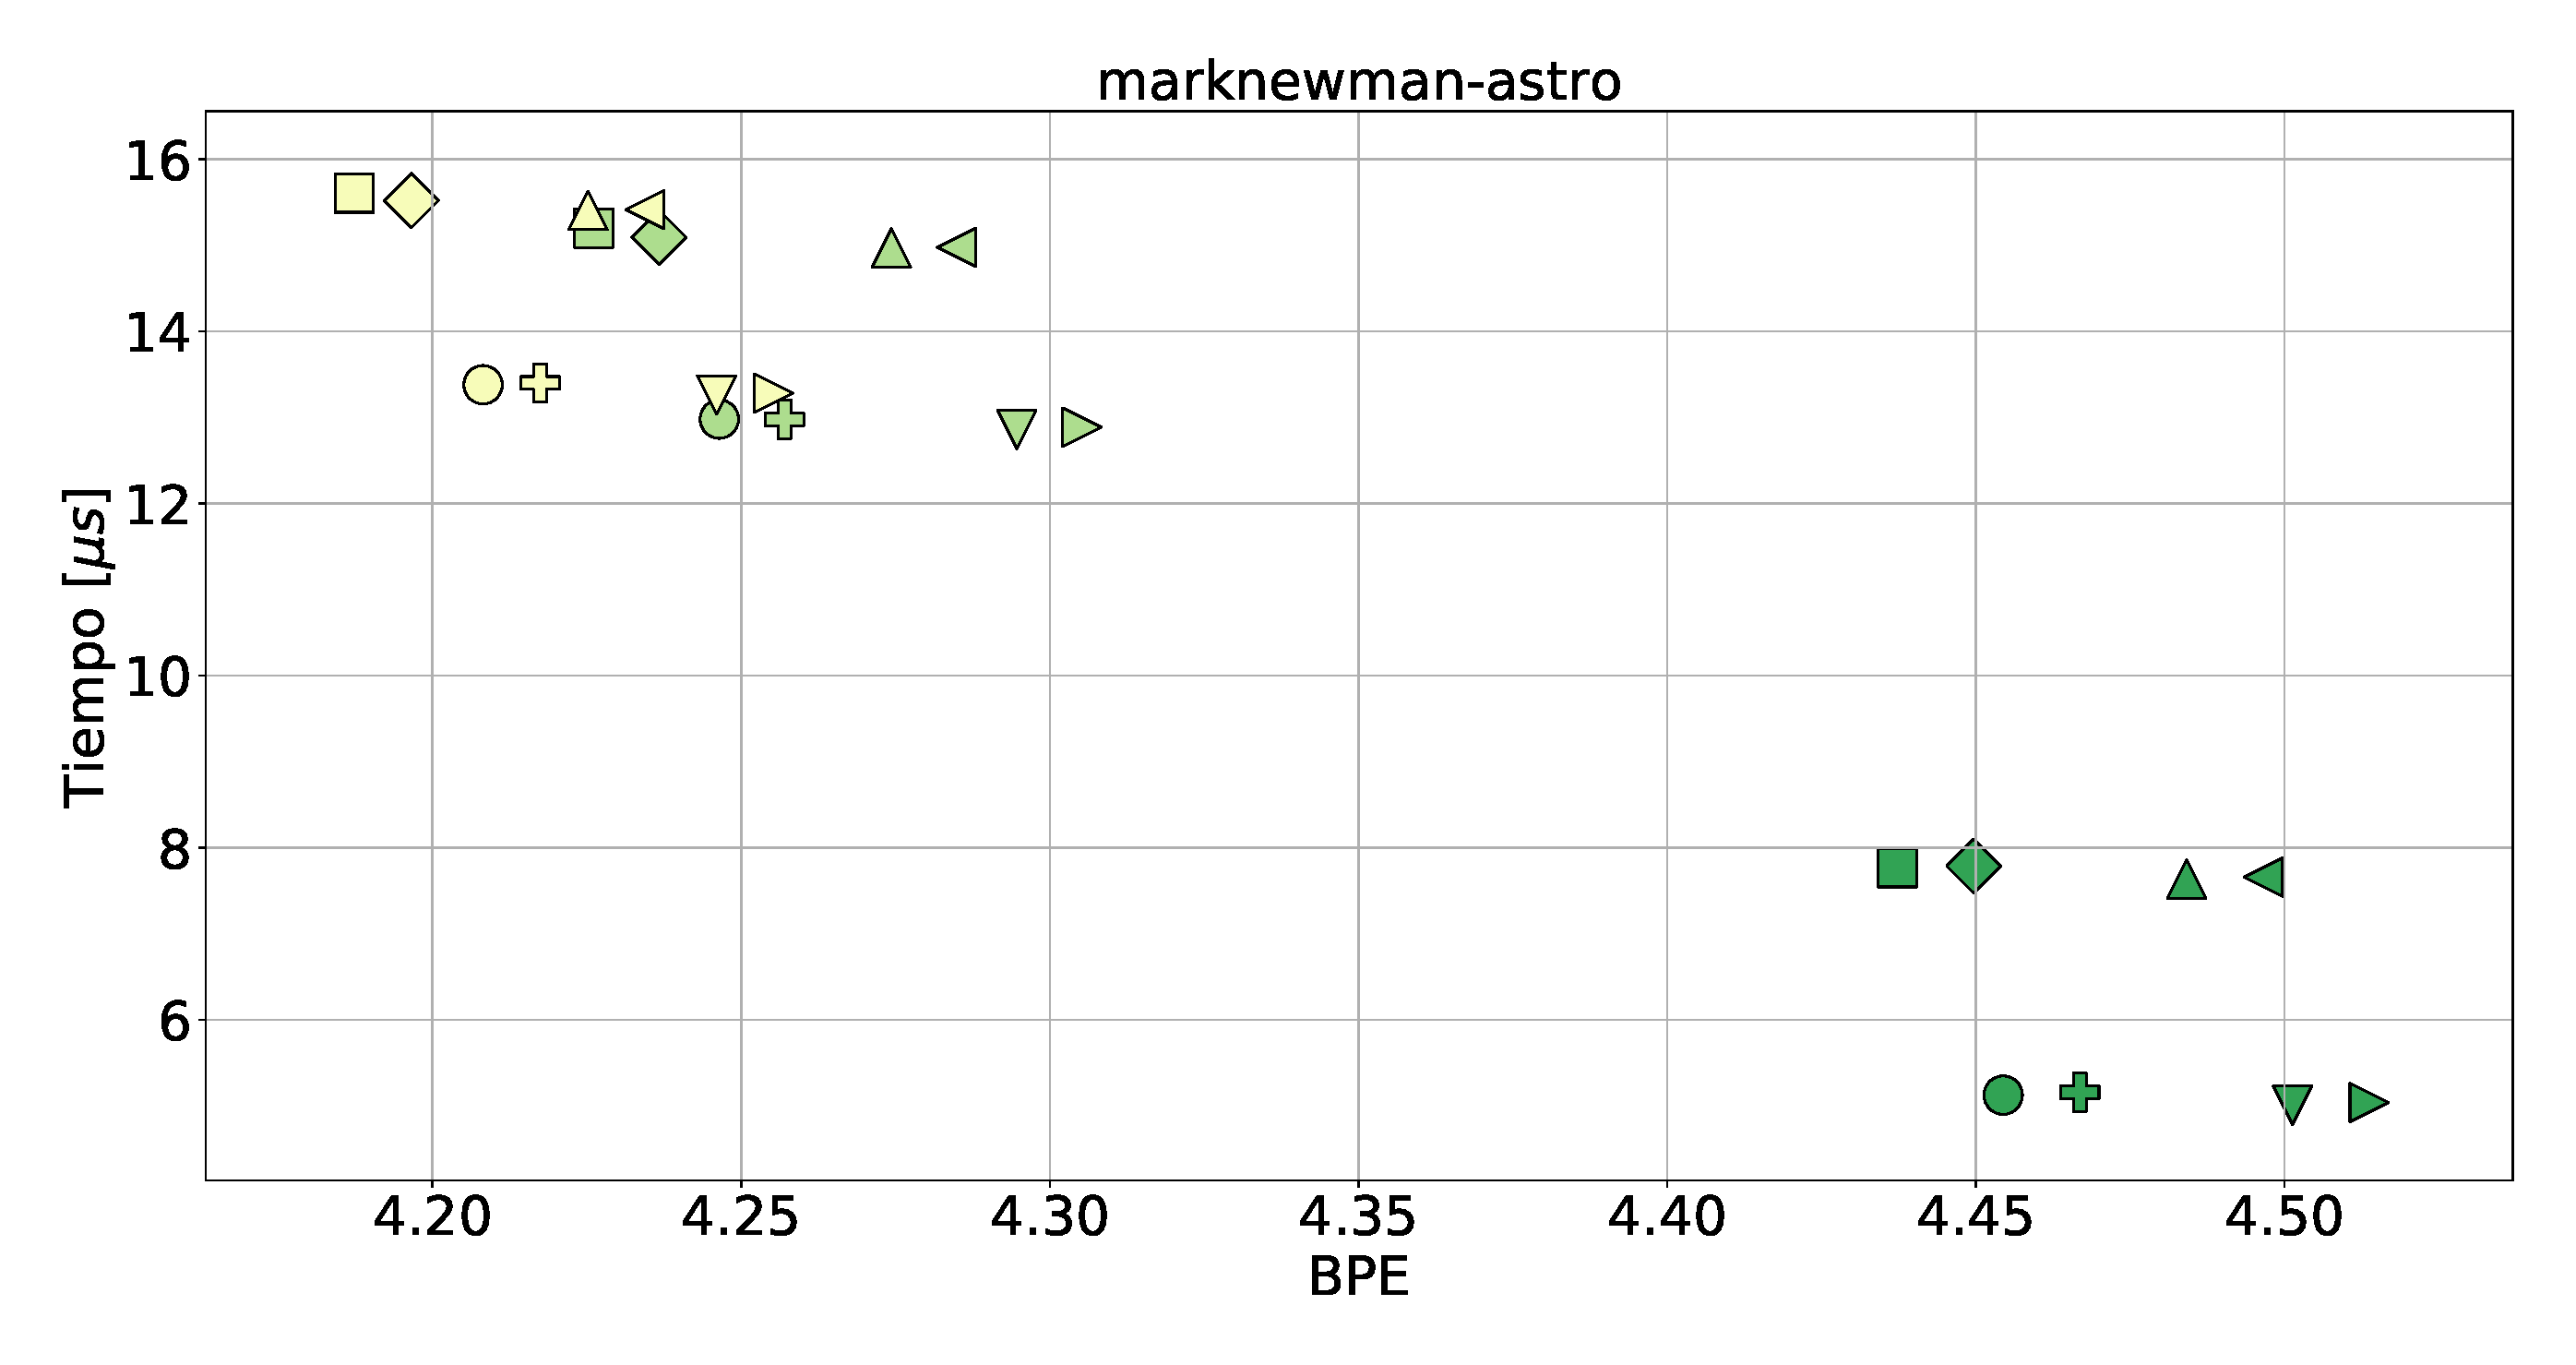
\includegraphics[width=1\linewidth]{../img/sdsl/aleatorioBig/marknewman-astro.pdf}
%    		\end{minipage}
%    		\begin{minipage}{0.15\textwidth}
%    			\centering
%    			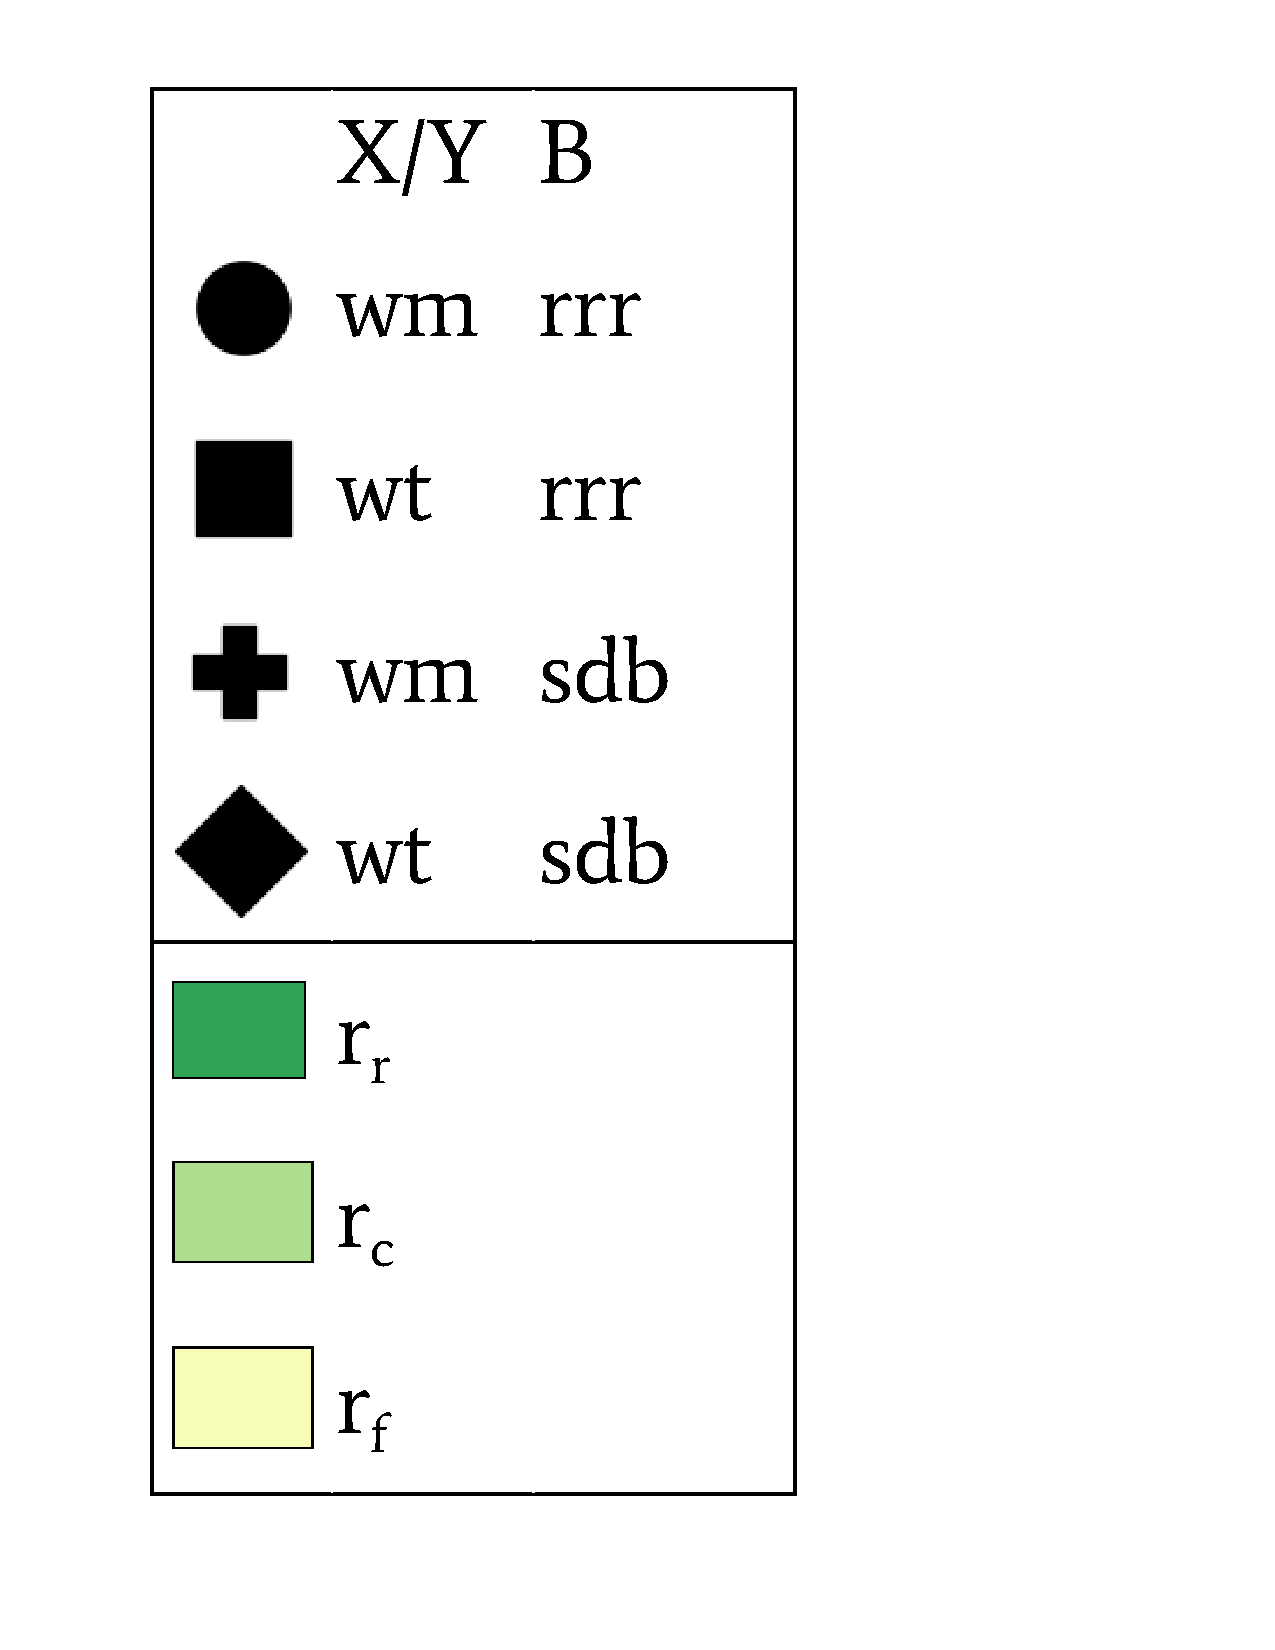
\includegraphics[scale=.15, clip, trim=70 0 0 0]{../img/sdsl/label.pdf}
%    		\end{minipage}	
%    	\end{minipage}
%
%	\caption{BPE y Tiempo de acceso aleatorio medio para posibles estructuras compactas, por cada función de ranking, para marknewman-astro.}
%\end{figure}
%
%\end{frame}





%%% Funciones de ranking
%\begin{frame}
%\frametitle{Resultados - Funciones de ranking}
%
%\begin{itemize}
%	\item $r_{f}(u)$: Frecuencia del vértice $u$ en cliques.
%	\item $r_{c}(u)$: Cantidad de vecinos en cliques de vértice $u$.
%	\item $r_{r}(u)$: Razón entre ambas funciones $r_{c}(u)/r_{f}(u)$.
%\end{itemize}
%
%\end{frame}


\begin{frame}
\frametitle{Resultados - Funciones de ranking}

\begin{table}
	\caption{Comparativa de BPE de las estructuras compactas para las funciones de ranking.}
	\rowcolors{2}{white}{gray!10}
	\label{table:bpe3}
	\centering
	\begin{tabular}{l|r|r|r}
		\toprule
		Grafo & $r_{r}$ & $r_{c}$ & $r_{f}$\\
		\midrule
		marknewman-astro & 3,96 & 3,86 & \textbf{3,82} \\
        marknewman-condmat & 5,74 & 5,47 & \textbf{5,44} \\
        dblp-2010 & 5,85 & 5,97 & \textbf{5,73} \\
        dblp-2011 & 6,58 & 6,63 & \textbf{6,48} \\
        snap-dblp & 6,89 & 6,50 & \textbf{6,41} \\
        snap-amazon & \textbf{10,44} & 10,53 & 10,46 \\
        coPapersDBLP & 0,78 & 0,79 & \textbf{0,76} \\
        coPapersCiteseer & 0,52 & 0,50 & \textbf{0,48} \\
        \bottomrule
	\end{tabular}
\end{table}


\end{frame}


\begin{frame}
\frametitle{Resultados - Funciones de ranking (2)}

\begin{figure}
    	\centering
    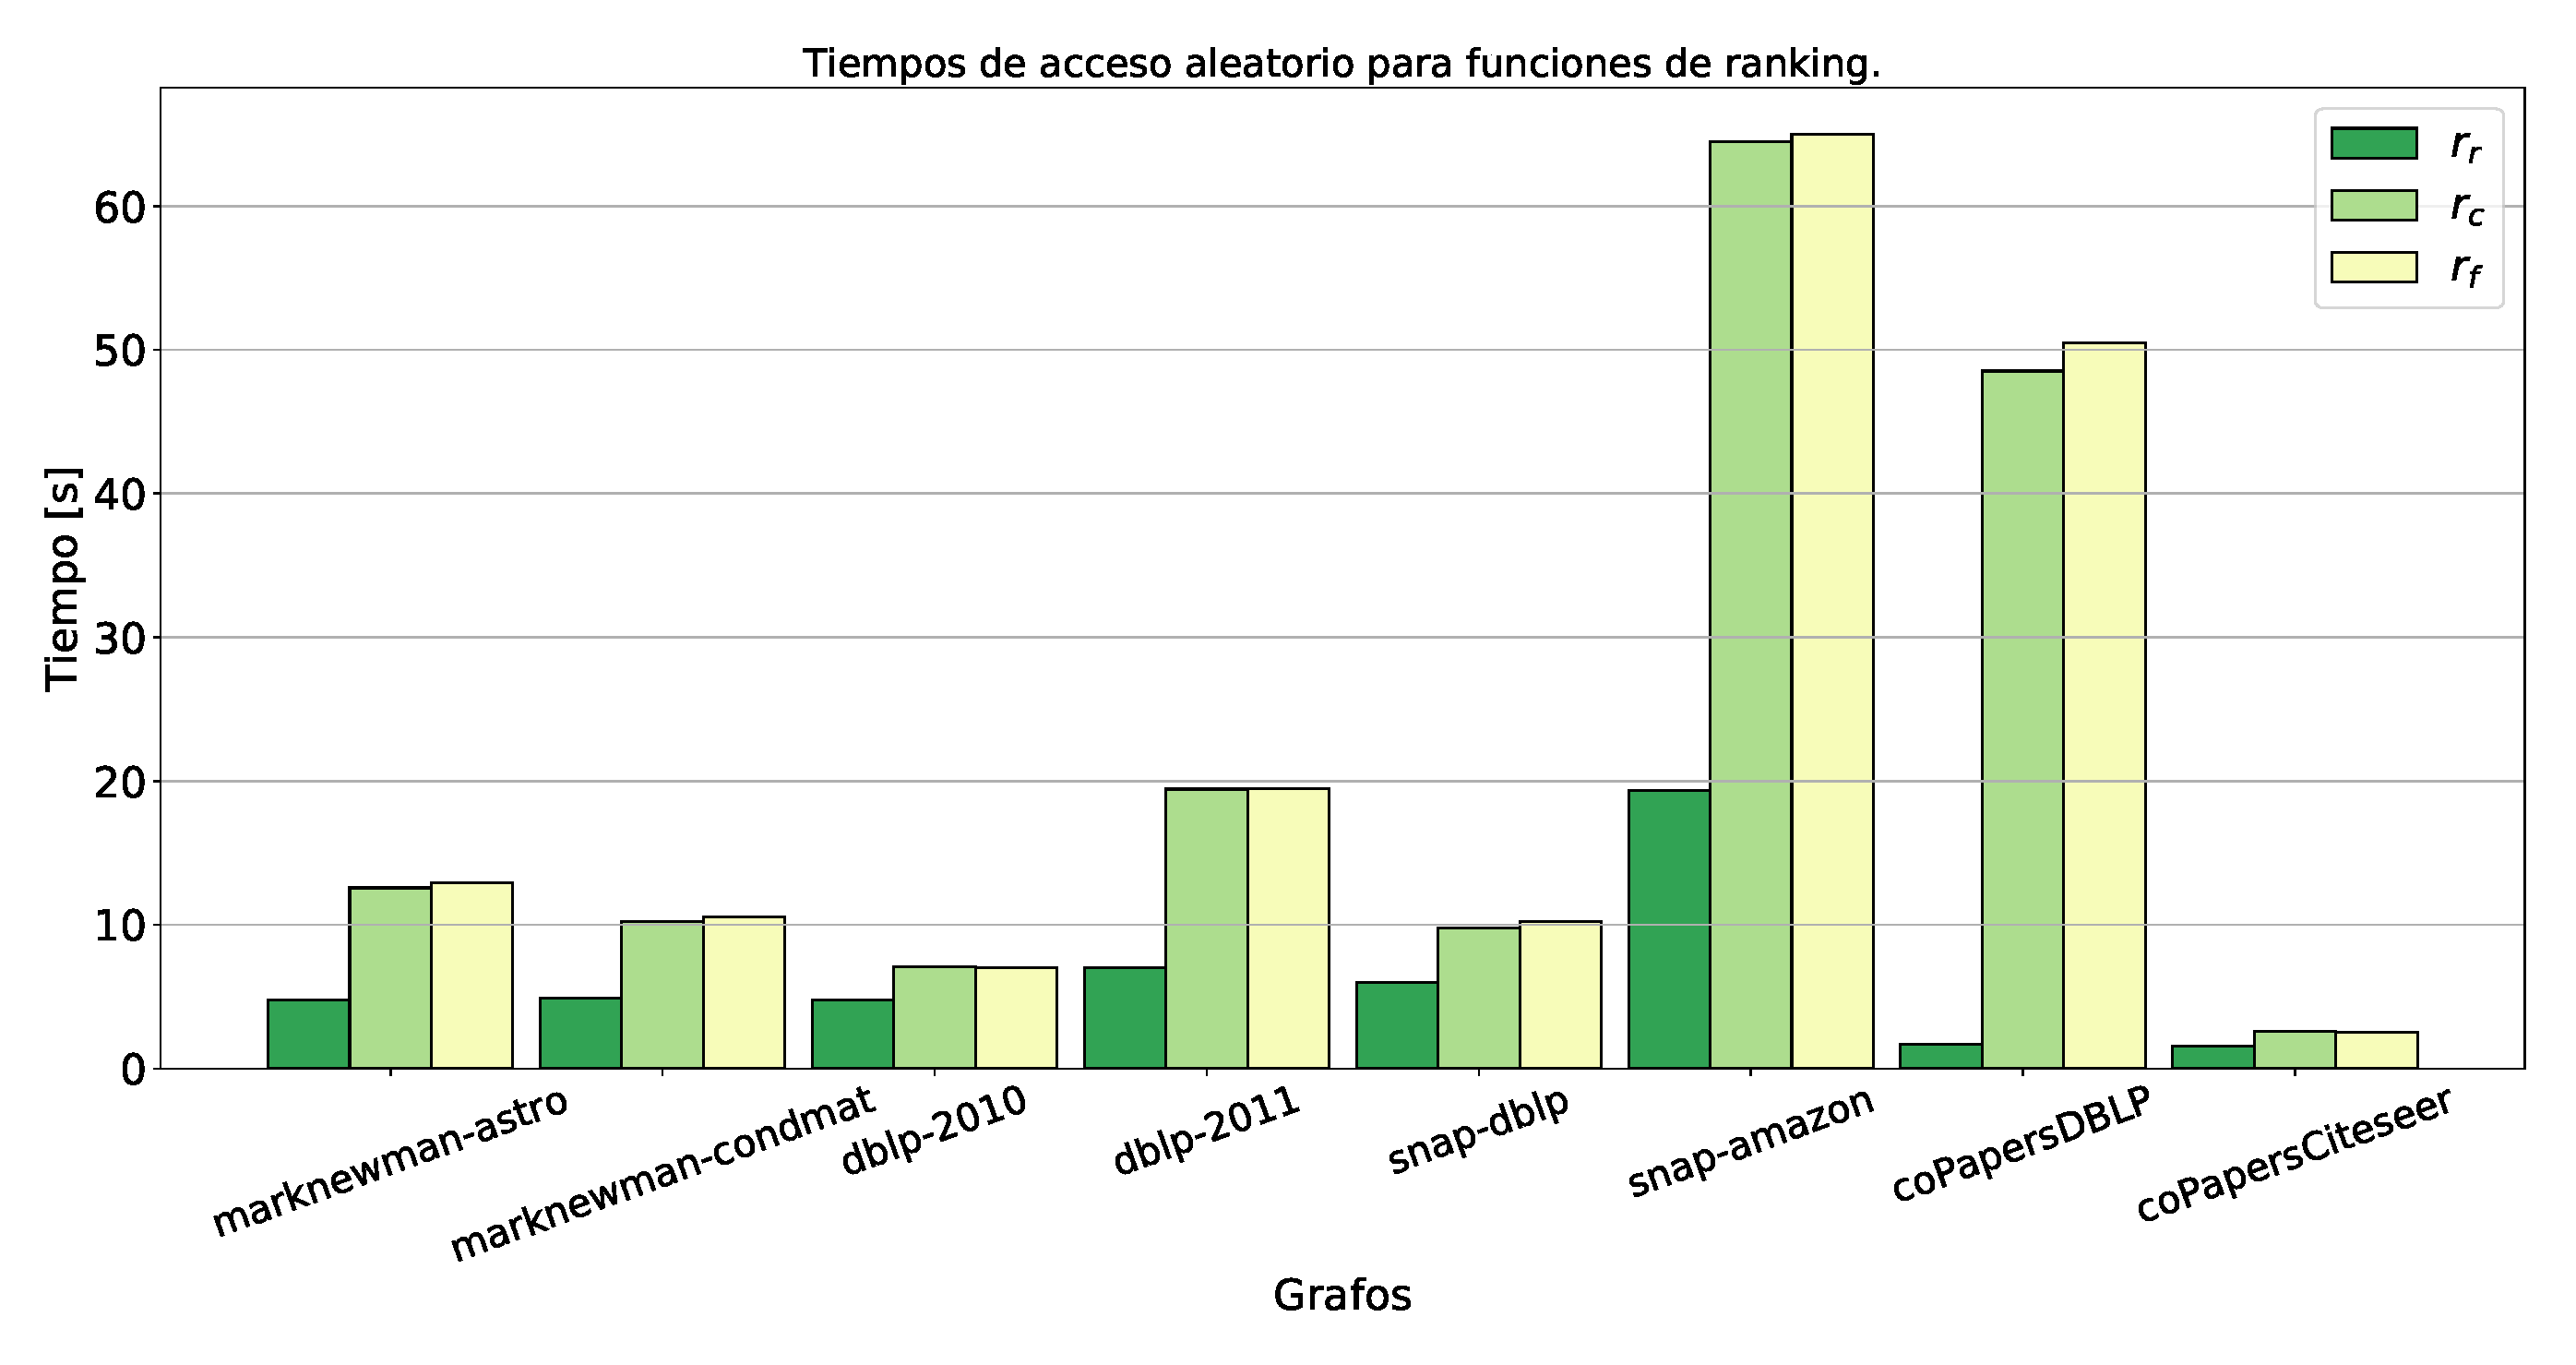
\includegraphics[width=1\linewidth]{../img/timesRanking.pdf}
    	
    \caption{Tiempos de acceso aleatorio para las funciones de ranking.}
\end{figure}

\end{frame}


\begin{frame}
\frametitle{Resultados - Tiempos de generación}

{\footnotesize
\begin{table}
	\caption{Tiempos de obtención de listado de cliques maximales y construcción de la estructura compacta, en segundos.}
	\rowcolors{2}{white}{gray!10}
	\label{table:constructTimes}
	\centering
	\begin{tabular}{l|r|r|r|r}
		\toprule
		Grafo & $t_{\mathcal{C}}$ & $t_{CS}$ & $t_{T}$ & $t'_{\mathcal{C}}$ \\
		\midrule
		marknewman-astro & 0,18 & 0,28 & 0,46 & 0,10  \\
		marknewman-condmat & 0,28 & 0,40 & 0,68 & 0,18 \\
		dblp-2010 & 1,12 & 1,46 & 2,58 & 0,76  \\
         dblp-2011 & 5,58 & 7,30 & 12,88 & 3,55 \\
		snap-dblp & 1,68 & 2,30 & 3,98 & 1,12 \\
         snap-amazon & 5,93 & 8,44 & 14,37 & 4,12 \\
         coPapersDBLP & 17,96 & 3,44 & 21,40 & 1,60 \\
         coPapersCiteseer & 26,70 & 4,70 & 31,40 & 1,12 \\
         \bottomrule
	\end{tabular}
\end{table}
}

$t_{\mathcal{C}}$: generación del listado de cliques maximales $\mathcal{C}$.

$t_{CS}$: generar la estructura compacta desde listado de cliques $\mathcal{C}$.

$t_{T} = t_{\mathcal{C}} + t_{CS}$

$t'_{\mathcal{C}}$: recuperar el listado de cliques $\mathcal{C}$.

\end{frame}

